Partiendo de las 3 tablas originales, la eliminación de variables, el agregado de los nuevos atributos y por último las transformaciones realizadas (todas vistas en las seciones anteriores), se genera un tablón principal. El mismo se llama \textbf{\textit{``baseline\_2009.csv"}}. \\

Dicho tablón también fue generado en el script \textit{``Giar 20-09.ipynb"} luego de hacer el preprocesamiento.

A continuación de presenta una muestra aleatoria pero invertiremos las filas por columnas para que entre en la hoja:

\begingroup\fontsize{10}{12}\selectfont

\begin{longtable}[t]{llll}
\caption{\label{tab:tabla_tablon_baseline}Ejemplo de Tablón}\\
\toprule
\rowcolor{black}  \multicolumn{1}{c}{\textcolor{white}{\textbf{variable}}} & \multicolumn{1}{c}{\textcolor{white}{\textbf{10000007}}} & \multicolumn{1}{c}{\textcolor{white}{\textbf{10000015}}} & \multicolumn{1}{c}{\textcolor{white}{\textbf{10000016}}}\\
\midrule
\endfirsthead
\caption[]{Ejemplo de Tablón \textit{(continued)}}\\
\toprule
\rowcolor{black}  \multicolumn{1}{c}{\textcolor{white}{\textbf{variable}}} & \multicolumn{1}{c}{\textcolor{white}{\textbf{10000007}}} & \multicolumn{1}{c}{\textcolor{white}{\textbf{10000015}}} & \multicolumn{1}{c}{\textcolor{white}{\textbf{10000016}}}\\
\midrule
\endhead
\
\endfoot
\bottomrule
\endlastfoot
\rowcolor{gray!6}  Aprobado & 2 & 14 & 5\\
Cantidad de veces recursada regular & 0 & 0 & 0\\
\rowcolor{gray!6}  Ciclo Lectivo de Cursada & 2014 & 2014 & 2014\\
Descripción de recursada regular\_No Recurso & 1 & 4 & 7\\
\rowcolor{gray!6}  Descripción de recursada regular\_Recurso 1 Vez & 0 & 0 & 0\\
\addlinespace
Descripción de recursada regular\_Recurso 2 Veces & 0 & 0 & 0\\
\rowcolor{gray!6}  Descripción de recursada regular\_Recurso 3 Veces & 0 & 0 & 0\\
Descripción de recursada regular\_Recurso 4 Veces & 0 & 0 & 0\\
\rowcolor{gray!6}  Descripción de recursada regular\_Recurso 5 Veces & 0 & 0 & 0\\
Descripción de recursada regular\_Recurso n Veces (>5) & 0 & 0 & 0\\
\addlinespace
\rowcolor{gray!6}  deserto & 1 & 1 & 1\\
edad al ingreso & 22 & 35 & 34\\
\rowcolor{gray!6}  EsTecnico & NA & NA & NA\\
noAprobado & 0 & 0 & 0\\
\rowcolor{gray!6}  Nota & 10 & 9 & 10\\
\addlinespace
Nota\_max\_prom & 10 & 9.92857142857143 & 10\\
\rowcolor{gray!6}  Promociono & 0 & 0 & 0\\
Sexo & M & M & M\\
\rowcolor{gray!6}  Tipo de aprobación\_Cambio Curso & 0 & 0 & 0\\
Tipo de aprobación\_Firmo & 0 & 1 & 0\\
\addlinespace
\rowcolor{gray!6}  Tipo de aprobación\_Libre & 0 & 3 & 6\\
Tipo de aprobación\_No Firmo & 1 & 1 & 1\\
\rowcolor{gray!6}  Tipo de aprobación\_Promociono & 0 & 0 & 0\\
Turno\_Mañana & 0 & 0 & 0\\
\rowcolor{gray!6}  Turno\_Noche & 1 & 4 & 6\\
\addlinespace
Turno\_Tarde & 0 & 1 & 1\\*
\end{longtable}
\endgroup{}





\todorevisar{vale la pena hacer estadisticos aca ? ahora son todos numericos (la mayoria)}

\subsection{Exploración de datos Integrados}

\hypertarget{anuxe1lisis-estaduxedstico}{%
	\subsubsection{Análisis Estadístico}\label{anuxe1lisis-estaduxedstico}}

A continuación se realiza un breve análisis estadístico sobre como
quedan los campos en el tablón ``Baseline\_2009'' después de la
integración de la información, agregación de campos y campos calculados:


\begin{table}[!h]
	
	\caption{\label{tab:tablon_est_cal}Tablón - Análisis Estadístico Numérico}
	\centering
	\resizebox{\linewidth}{!}{
		\begin{tabular}[t]{llrrrrrr}
			\toprule
			\rowcolor{black}  \multicolumn{1}{c}{\textcolor{white}{\textbf{variable}}} & \multicolumn{1}{c}{\textcolor{white}{\textbf{tipo}}} & \multicolumn{1}{c}{\textcolor{white}{\textbf{observaciones}}} & \multicolumn{1}{c}{\textcolor{white}{\textbf{observaciones\_pct}}} & \multicolumn{1}{c}{\textcolor{white}{\textbf{nulos}}} & \multicolumn{1}{c}{\textcolor{white}{\textbf{nulos\_pct}}} & \multicolumn{1}{c}{\textcolor{white}{\textbf{valores\_unicos}}} & \multicolumn{1}{c}{\textcolor{white}{\textbf{valores\_unicos\_pct}}}\\
			\midrule
			\rowcolor{gray!6}  Turno\_Manana & numeric & 4558 & 100.00 & 0 & 0.00 & 42 & 0.92\\
			tipo\_de\_aprobacion\_libre & numeric & 4558 & 100.00 & 0 & 0.00 & 29 & 0.64\\
			\rowcolor{gray!6}  tipo\_de\_aprobacion\_cambio\_curso & numeric & 4558 & 100.00 & 0 & 0.00 & 18 & 0.39\\
			tipo\_de\_aprobacion\_promociono & numeric & 4558 & 100.00 & 0 & 0.00 & 10 & 0.22\\
			\rowcolor{gray!6}  edad\_al\_ingreso & numeric & 4558 & 100.00 & 0 & 0.00 & 39 & 0.86\\
			\addlinespace
			tipo\_de\_aprobacion\_no\_firmo & numeric & 4558 & 100.00 & 0 & 0.00 & 31 & 0.68\\
			\rowcolor{gray!6}  ciclo\_lectivo\_de\_cursada & numeric & 4558 & 100.00 & 0 & 0.00 & 7 & 0.15\\
			tipo\_de\_aprobacion\_firmo & numeric & 4558 & 100.00 & 0 & 0.00 & 41 & 0.90\\
			\rowcolor{gray!6}  cant\_resursada\_regular & numeric & 4558 & 100.00 & 0 & 0.00 & 42 & 0.92\\
			cant\_recursada\_regular\_No\_Recurso & numeric & 4558 & 100.00 & 0 & 0.00 & 46 & 1.01\\
			\addlinespace
			\rowcolor{gray!6}  cant\_recursada\_regular\_Recurso1vez & numeric & 4558 & 100.00 & 0 & 0.00 & 13 & 0.29\\
			cant\_recursada\_regular\_Recurso2vez & numeric & 4558 & 100.00 & 0 & 0.00 & 7 & 0.15\\
			\rowcolor{gray!6}  cant\_recursada\_regular\_Recurso3vez & numeric & 4558 & 100.00 & 0 & 0.00 & 5 & 0.11\\
			cant\_recursada\_regular\_Recurso4vez & numeric & 4558 & 100.00 & 0 & 0.00 & 4 & 0.09\\
			\rowcolor{gray!6}  cant\_recursada\_regular\_Recurso5vez & numeric & 4558 & 100.00 & 0 & 0.00 & 3 & 0.07\\
			\addlinespace
			cant\_recursada\_regular\_RecursoNveces & numeric & 4558 & 100.00 & 0 & 0.00 & 4 & 0.09\\
			\rowcolor{gray!6}  EsTecnico & character & 3951 & 86.68 & 607 & 13.32 & 3 & 0.07\\
			deserto & character & 4558 & 100.00 & 0 & 0.00 & 2 & 0.04\\
			\rowcolor{gray!6}  Sexo & character & 4558 & 100.00 & 0 & 0.00 & 2 & 0.04\\
			Turno\_Tarde & numeric & 4558 & 100.00 & 0 & 0.00 & 23 & 0.50\\
			\addlinespace
			\rowcolor{gray!6}  Turno\_Noche & numeric & 4558 & 100.00 & 0 & 0.00 & 42 & 0.92\\
			Aprobado & numeric & 4558 & 100.00 & 0 & 0.00 & 47 & 1.03\\
			\rowcolor{gray!6}  Promociono & numeric & 4558 & 100.00 & 0 & 0.00 & 10 & 0.22\\
			noAprobado & numeric & 4558 & 100.00 & 0 & 0.00 & 19 & 0.42\\
			\rowcolor{gray!6}  Nota & numeric & 4558 & 100.00 & 0 & 0.00 & 10 & 0.22\\
			\addlinespace
			Nota\_max\_prom & numeric & 4558 & 100.00 & 0 & 0.00 & 778 & 17.07\\
			\bottomrule
	\end{tabular}}
\end{table}


\begin{table}[!h]
	
	\caption{\label{tab:tablon_est_cat}Tablón Análisis Estadístico categóricas}
	\centering
	%\resizebox{\linewidth}{!}{
		\begin{tabular}[t]{llrrr}
			\toprule
			\rowcolor{black}  \multicolumn{1}{c}{\textcolor{white}{\textbf{variable}}} & \multicolumn{1}{c}{\textcolor{white}{\textbf{característica}}} & \multicolumn{1}{c}{\textcolor{white}{\textbf{frecuencia}}} & \multicolumn{1}{c}{\textcolor{white}{\textbf{frecuencia\_pct}}} & \multicolumn{1}{c}{\textcolor{white}{\textbf{rank}}}\\
			\midrule
			\rowcolor{gray!6}  EsTecnico & 0 & 2794 & 61.30 & 1\\
			EsTecnico & 1 & 1157 & 25.38 & 2\\
			\rowcolor{gray!6}  EsTecnico & NA & 607 & 13.32 & 3\\
			deserto & 0 & 2558 & 56.12 & 1\\
			\rowcolor{gray!6}  deserto & 1 & 2000 & 43.88 & 2\\
			\addlinespace
			Sexo & M & 3941 & 86.46 & 1\\
			\rowcolor{gray!6}  Sexo & F & 617 & 13.54 & 2\\
			\bottomrule
	\end{tabular}%}
\end{table}

\begin{table}[!h]
	
	\caption{\label{tab:tablon_est_num1}Tablón Análisis Estadístico Numérico}
	\centering
	\resizebox{\linewidth}{!}{
		\begin{tabular}[t]{lrrrrrrrrr}
			\toprule
			\rowcolor{black}  \multicolumn{1}{c}{\textcolor{white}{\textbf{variable}}} & \multicolumn{1}{c}{\textcolor{white}{\textbf{promedio}}} & \multicolumn{1}{c}{\textcolor{white}{\textbf{desvío}}} & \multicolumn{1}{c}{\textcolor{white}{\textbf{minimo}}} & \multicolumn{1}{c}{\textcolor{white}{\textbf{maximo}}} & \multicolumn{1}{c}{\textcolor{white}{\textbf{P05}}} & \multicolumn{1}{c}{\textcolor{white}{\textbf{Q1}}} & \multicolumn{1}{c}{\textcolor{white}{\textbf{mediana}}} & \multicolumn{1}{c}{\textcolor{white}{\textbf{Q3}}} & \multicolumn{1}{c}{\textcolor{white}{\textbf{P95}}}\\
			\midrule
			\rowcolor{gray!6}  Turno\_Manana & 10.35 & 8.07 & 0 & 42 & 0.00 & 3.00 & 9.00 & 16 & 25\\
			tipo\_de\_aprobacion\_libre & 3.49 & 3.68 & 0 & 32 & 0.00 & 1.00 & 2.00 & 5 & 11\\
			\rowcolor{gray!6}  tipo\_de\_aprobacion\_cambio\_curso & 1.35 & 2.41 & 0 & 17 & 0.00 & 0.00 & 0.00 & 1 & 7\\
			tipo\_de\_aprobacion\_promociono & 1.82 & 1.93 & 0 & 9 & 0.00 & 0.00 & 1.00 & 3 & 6\\
			\rowcolor{gray!6}  edad\_al\_ingreso & 20.25 & 3.50 & 11 & 58 & 18.00 & 18.00 & 19.00 & 20 & 27\\
			\addlinespace
			tipo\_de\_aprobacion\_no\_firmo & 6.05 & 4.66 & 0 & 34 & 0.00 & 2.00 & 5.00 & 9 & 15\\
			\rowcolor{gray!6}  ciclo\_lectivo\_de\_cursada & 2013.26 & 1.40 & 2008 & 2014 & 2010.00 & 2013.00 & 2014.00 & 2014 & 2014\\
			tipo\_de\_aprobacion\_firmo & 9.83 & 8.83 & 0 & 40 & 1.00 & 4.00 & 7.00 & 14 & 29\\
			\rowcolor{gray!6}  cant\_resursada\_regular & 5.26 & 13.34 & 0 & 298 & 0.00 & 0.00 & 3.00 & 7 & 13\\
			cant\_recursada\_regular\_No\_Recurso & 12.05 & 8.90 & 0 & 45 & 3.00 & 6.00 & 8.00 & 15 & 33\\
			\addlinespace
			\rowcolor{gray!6}  cant\_recursada\_regular\_Recurso1vez & 2.04 & 1.89 & 0 & 12 & 0.00 & 0.00 & 2.00 & 3 & 6\\
			cant\_recursada\_regular\_Recurso2vez & 0.58 & 0.92 & 0 & 7 & 0.00 & 0.00 & 0.00 & 1 & 2\\
			\rowcolor{gray!6}  cant\_recursada\_regular\_Recurso3vez & 0.19 & 0.50 & 0 & 4 & 0.00 & 0.00 & 0.00 & 0 & 1\\
			cant\_recursada\_regular\_Recurso4vez & 0.07 & 0.29 & 0 & 3 & 0.00 & 0.00 & 0.00 & 0 & 1\\
			\rowcolor{gray!6}  cant\_recursada\_regular\_Recurso5vez & 0.02 & 0.16 & 0 & 2 & 0.00 & 0.00 & 0.00 & 0 & 0\\
			\addlinespace
			cant\_recursada\_regular\_RecursoNveces & 0.01 & 0.12 & 0 & 3 & 0.00 & 0.00 & 0.00 & 0 & 0\\
			\rowcolor{gray!6}  Turno\_Tarde & 4.48 & 4.17 & 0 & 22 & 0.00 & 1.00 & 3.00 & 7 & 12\\
			Turno\_Noche & 7.71 & 7.81 & 0 & 45 & 0.00 & 1.00 & 5.00 & 13 & 23\\
			\rowcolor{gray!6}  Aprobado & 9.56 & 10.23 & 0 & 46 & 1.00 & 2.00 & 6.00 & 13 & 34\\
			Promociono & 1.84 & 1.93 & 0 & 9 & 0.00 & 0.00 & 1.00 & 3 & 6\\
			\addlinespace
			\rowcolor{gray!6}  noAprobado & 2.28 & 2.67 & 0 & 19 & 0.00 & 0.00 & 1.00 & 3 & 8\\
			Nota & 5.37 & 1.72 & 1 & 10 & 3.00 & 4.00 & 5.00 & 6 & 9\\
			\rowcolor{gray!6}  Nota\_max\_prom & 6.13 & 1.62 & 1 & 10 & 3.33 & 5.25 & 6.17 & 7 & 9\\
			\bottomrule
	\end{tabular}}
\end{table}


\begin{table}[!h]
	
	\caption{\label{tab:tablon_est_num2}Tablón Análisis Estadístico Numérico}
	\centering
	\resizebox{\linewidth}{!}{
		\begin{tabular}[t]{lrrrrrr}
			\toprule
			\rowcolor{black}  \multicolumn{1}{c}{\textcolor{white}{\textbf{variable}}} & \multicolumn{1}{c}{\textcolor{white}{\textbf{ceros}}} & \multicolumn{1}{c}{\textcolor{white}{\textbf{ceros\_pct}}} & \multicolumn{1}{c}{\textcolor{white}{\textbf{negativos}}} & \multicolumn{1}{c}{\textcolor{white}{\textbf{negativos\_pct}}} & \multicolumn{1}{c}{\textcolor{white}{\textbf{outliers}}} & \multicolumn{1}{c}{\textcolor{white}{\textbf{outliers\_pct}}}\\
			\midrule
			\rowcolor{gray!6}  Turno\_Manana & 506 & 11.10 & 0 & 0 & 7 & 0.15\\
			tipo\_de\_aprobacion\_libre & 869 & 19.07 & 0 & 0 & 179 & 3.93\\
			\rowcolor{gray!6}  tipo\_de\_aprobacion\_cambio\_curso & 2607 & 57.20 & 0 & 0 & 794 & 17.42\\
			tipo\_de\_aprobacion\_promociono & 1462 & 32.08 & 0 & 0 & 34 & 0.75\\
			\rowcolor{gray!6}  edad\_al\_ingreso & 0 & 0.00 & 0 & 0 & 499 & 10.95\\
			\addlinespace
			tipo\_de\_aprobacion\_no\_firmo & 362 & 7.94 & 0 & 0 & 54 & 1.18\\
			\rowcolor{gray!6}  ciclo\_lectivo\_de\_cursada & 0 & 0.00 & 0 & 0 & 606 & 13.30\\
			tipo\_de\_aprobacion\_firmo & 159 & 3.49 & 0 & 0 & 227 & 4.98\\
			\rowcolor{gray!6}  cant\_resursada\_regular & 1149 & 25.21 & 0 & 0 & 71 & 1.56\\
			cant\_recursada\_regular\_No\_Recurso & 5 & 0.11 & 0 & 0 & 331 & 7.26\\
			\addlinespace
			\rowcolor{gray!6}  cant\_recursada\_regular\_Recurso1vez & 1271 & 27.89 & 0 & 0 & 35 & 0.77\\
			cant\_recursada\_regular\_Recurso2vez & 2908 & 63.80 & 0 & 0 & 219 & 4.80\\
			\rowcolor{gray!6}  cant\_recursada\_regular\_Recurso3vez & 3885 & 85.23 & 0 & 0 & 673 & 14.77\\
			cant\_recursada\_regular\_Recurso4vez & 4288 & 94.08 & 0 & 0 & 270 & 5.92\\
			\rowcolor{gray!6}  cant\_recursada\_regular\_Recurso5vez & 4459 & 97.83 & 0 & 0 & 99 & 2.17\\
			\addlinespace
			cant\_recursada\_regular\_RecursoNveces & 4516 & 99.08 & 0 & 0 & 42 & 0.92\\
			\rowcolor{gray!6}  Turno\_Tarde & 875 & 19.20 & 0 & 0 & 34 & 0.75\\
			Turno\_Noche & 911 & 19.99 & 0 & 0 & 36 & 0.79\\
			\rowcolor{gray!6}  Aprobado & 157 & 3.44 & 0 & 0 & 297 & 6.52\\
			Promociono & 1441 & 31.61 & 0 & 0 & 34 & 0.75\\
			\addlinespace
			\rowcolor{gray!6}  noAprobado & 1353 & 29.68 & 0 & 0 & 248 & 5.44\\
			Nota & 0 & 0.00 & 0 & 0 & 143 & 3.14\\
			\rowcolor{gray!6}  Nota\_max\_prom & 0 & 0.00 & 0 & 0 & 321 & 7.04\\
			\bottomrule
	\end{tabular}}
\end{table}


\clearpage

\hypertarget{dataset-supervisado-valores-en-funciuxf3n-de-la-clase}{%
	\subparagraph{Dataset Supervisado: Valores en función de la
		clase}\label{dataset-supervisado-valores-en-funciuxf3n-de-la-clase}}

Como es un dataset supervisado, podría ser interesante ver los valores
separados por clase. Por lo tanto el dataset y con el objeto solamente
de realizar un análisis exploratorio, se divide según la clase y se
realizan los estadísticos nuevamente.

\begin{table}[!h]
	
	\caption{\label{tab:tablon_no_deserto_est_cal}Tablón NO Desertores - Análisis Estadístico Numérico}
	\centering
	\resizebox{\linewidth}{!}{
		\begin{tabular}[t]{llrrrrrr}
			\toprule
			\rowcolor{black}  \multicolumn{1}{c}{\textcolor{white}{\textbf{variable}}} & \multicolumn{1}{c}{\textcolor{white}{\textbf{tipo}}} & \multicolumn{1}{c}{\textcolor{white}{\textbf{observaciones}}} & \multicolumn{1}{c}{\textcolor{white}{\textbf{observaciones\_pct}}} & \multicolumn{1}{c}{\textcolor{white}{\textbf{nulos}}} & \multicolumn{1}{c}{\textcolor{white}{\textbf{nulos\_pct}}} & \multicolumn{1}{c}{\textcolor{white}{\textbf{valores\_unicos}}} & \multicolumn{1}{c}{\textcolor{white}{\textbf{valores\_unicos\_pct}}}\\
			\midrule
			\rowcolor{gray!6}  Turno\_Manana & numeric & 2558 & 100.00 & 0 & 0.00 & 42 & 1.64\\
			tipo\_de\_aprobacion\_libre & numeric & 2558 & 100.00 & 0 & 0.00 & 23 & 0.90\\
			\rowcolor{gray!6}  tipo\_de\_aprobacion\_cambio\_curso & numeric & 2558 & 100.00 & 0 & 0.00 & 16 & 0.63\\
			tipo\_de\_aprobacion\_promociono & numeric & 2558 & 100.00 & 0 & 0.00 & 10 & 0.39\\
			\rowcolor{gray!6}  edad\_al\_ingreso & numeric & 2558 & 100.00 & 0 & 0.00 & 27 & 1.06\\
			\addlinespace
			tipo\_de\_aprobacion\_no\_firmo & numeric & 2558 & 100.00 & 0 & 0.00 & 29 & 1.13\\
			\rowcolor{gray!6}  ciclo\_lectivo\_de\_cursada & numeric & 2558 & 100.00 & 0 & 0.00 & 7 & 0.27\\
			tipo\_de\_aprobacion\_firmo & numeric & 2558 & 100.00 & 0 & 0.00 & 41 & 1.60\\
			\rowcolor{gray!6}  cant\_resursada\_regular & numeric & 2558 & 100.00 & 0 & 0.00 & 34 & 1.33\\
			cant\_recursada\_regular\_No\_Recurso & numeric & 2558 & 100.00 & 0 & 0.00 & 46 & 1.80\\
			\addlinespace
			\rowcolor{gray!6}  cant\_recursada\_regular\_Recurso1vez & numeric & 2558 & 100.00 & 0 & 0.00 & 13 & 0.51\\
			cant\_recursada\_regular\_Recurso2vez & numeric & 2558 & 100.00 & 0 & 0.00 & 7 & 0.27\\
			\rowcolor{gray!6}  cant\_recursada\_regular\_Recurso3vez & numeric & 2558 & 100.00 & 0 & 0.00 & 4 & 0.16\\
			cant\_recursada\_regular\_Recurso4vez & numeric & 2558 & 100.00 & 0 & 0.00 & 3 & 0.12\\
			\rowcolor{gray!6}  cant\_recursada\_regular\_Recurso5vez & numeric & 2558 & 100.00 & 0 & 0.00 & 3 & 0.12\\
			\addlinespace
			cant\_recursada\_regular\_RecursoNveces & numeric & 2558 & 100.00 & 0 & 0.00 & 3 & 0.12\\
			\rowcolor{gray!6}  EsTecnico & character & 2312 & 90.38 & 246 & 9.62 & 3 & 0.12\\
			deserto & character & 2558 & 100.00 & 0 & 0.00 & 1 & 0.04\\
			\rowcolor{gray!6}  Sexo & character & 2558 & 100.00 & 0 & 0.00 & 2 & 0.08\\
			Turno\_Tarde & numeric & 2558 & 100.00 & 0 & 0.00 & 22 & 0.86\\
			\addlinespace
			\rowcolor{gray!6}  Turno\_Noche & numeric & 2558 & 100.00 & 0 & 0.00 & 42 & 1.64\\
			Aprobado & numeric & 2558 & 100.00 & 0 & 0.00 & 47 & 1.84\\
			\rowcolor{gray!6}  Promociono & numeric & 2558 & 100.00 & 0 & 0.00 & 10 & 0.39\\
			noAprobado & numeric & 2558 & 100.00 & 0 & 0.00 & 19 & 0.74\\
			\rowcolor{gray!6}  Nota & numeric & 2558 & 100.00 & 0 & 0.00 & 10 & 0.39\\
			\addlinespace
			Nota\_max\_prom & numeric & 2558 & 100.00 & 0 & 0.00 & 718 & 28.07\\
			\bottomrule
	\end{tabular}}
\end{table}


\begin{table}[!h]
	
	\caption{\label{tab:tablon_no_deserto_est_cat}Tablón NO Desertores - Análisis Estadístico categóricas}
	\centering
	%\resizebox{\linewidth}{!}{
		\begin{tabular}[t]{llrrr}
			\toprule
			\rowcolor{black}  \multicolumn{1}{c}{\textcolor{white}{\textbf{variable}}} & \multicolumn{1}{c}{\textcolor{white}{\textbf{característica}}} & \multicolumn{1}{c}{\textcolor{white}{\textbf{frecuencia}}} & \multicolumn{1}{c}{\textcolor{white}{\textbf{frecuencia\_pct}}} & \multicolumn{1}{c}{\textcolor{white}{\textbf{rank}}}\\
			\midrule
			\rowcolor{gray!6}  EsTecnico & 0 & 1631 & 63.76 & 1\\
			EsTecnico & 1 & 681 & 26.62 & 2\\
			\rowcolor{gray!6}  EsTecnico & NA & 246 & 9.62 & 3\\
			deserto & 0 & 2558 & 100.00 & 1\\
			\rowcolor{gray!6}  Sexo & M & 2184 & 85.38 & 1\\
			\addlinespace
			Sexo & F & 374 & 14.62 & 2\\
			\bottomrule
	\end{tabular}%}
\end{table}


\begin{table}[!h]
	
	\caption{\label{tab:tablon_no_deserto_est_num1}Tablón NO Desertores - Análisis Estadístico Numérico}
	\centering
	\resizebox{\linewidth}{!}{
		\begin{tabular}[t]{lrrrrrrrrr}
			\toprule
			\rowcolor{black}  \multicolumn{1}{c}{\textcolor{white}{\textbf{variable}}} & \multicolumn{1}{c}{\textcolor{white}{\textbf{promedio}}} & \multicolumn{1}{c}{\textcolor{white}{\textbf{desvío}}} & \multicolumn{1}{c}{\textcolor{white}{\textbf{minimo}}} & \multicolumn{1}{c}{\textcolor{white}{\textbf{maximo}}} & \multicolumn{1}{c}{\textcolor{white}{\textbf{P05}}} & \multicolumn{1}{c}{\textcolor{white}{\textbf{Q1}}} & \multicolumn{1}{c}{\textcolor{white}{\textbf{mediana}}} & \multicolumn{1}{c}{\textcolor{white}{\textbf{Q3}}} & \multicolumn{1}{c}{\textcolor{white}{\textbf{P95}}}\\
			\midrule
			\rowcolor{gray!6}  Turno\_Manana & 12.09 & 8.48 & 0 & 42 & 0.00 & 5.00 & 12.00 & 19 & 26.00\\
			tipo\_de\_aprobacion\_libre & 2.58 & 3.08 & 0 & 30 & 0.00 & 0.00 & 2.00 & 4 & 8.00\\
			\rowcolor{gray!6}  tipo\_de\_aprobacion\_cambio\_curso & 1.58 & 2.55 & 0 & 17 & 0.00 & 0.00 & 0.00 & 2 & 7.00\\
			tipo\_de\_aprobacion\_promociono & 2.58 & 2.02 & 0 & 9 & 0.00 & 1.00 & 2.00 & 4 & 6.00\\
			\rowcolor{gray!6}  edad\_al\_ingreso & 19.78 & 2.86 & 16 & 49 & 18.00 & 18.00 & 19.00 & 20 & 25.00\\
			\addlinespace
			tipo\_de\_aprobacion\_no\_firmo & 5.58 & 4.70 & 0 & 34 & 0.00 & 2.00 & 5.00 & 8 & 14.00\\
			\rowcolor{gray!6}  ciclo\_lectivo\_de\_cursada & 2013.94 & 0.34 & 2008 & 2014 & 2014.00 & 2014.00 & 2014.00 & 2014 & 2014.00\\
			tipo\_de\_aprobacion\_firmo & 13.11 & 9.52 & 0 & 40 & 2.00 & 5.00 & 11.00 & 19 & 34.00\\
			\rowcolor{gray!6}  cant\_resursada\_regular & 4.66 & 11.11 & 0 & 216 & 0.00 & 0.00 & 3.00 & 6 & 13.00\\
			cant\_recursada\_regular\_No\_Recurso & 15.15 & 9.83 & 0 & 45 & 5.00 & 8.00 & 12.00 & 20 & 38.00\\
			\addlinespace
			\rowcolor{gray!6}  cant\_recursada\_regular\_Recurso1vez & 2.07 & 2.03 & 0 & 12 & 0.00 & 0.00 & 2.00 & 3 & 6.00\\
			cant\_recursada\_regular\_Recurso2vez & 0.55 & 0.93 & 0 & 7 & 0.00 & 0.00 & 0.00 & 1 & 2.00\\
			\rowcolor{gray!6}  cant\_recursada\_regular\_Recurso3vez & 0.17 & 0.46 & 0 & 3 & 0.00 & 0.00 & 0.00 & 0 & 1.00\\
			cant\_recursada\_regular\_Recurso4vez & 0.05 & 0.23 & 0 & 2 & 0.00 & 0.00 & 0.00 & 0 & 0.00\\
			\rowcolor{gray!6}  cant\_recursada\_regular\_Recurso5vez & 0.02 & 0.15 & 0 & 2 & 0.00 & 0.00 & 0.00 & 0 & 0.00\\
			\addlinespace
			cant\_recursada\_regular\_RecursoNveces & 0.01 & 0.10 & 0 & 2 & 0.00 & 0.00 & 0.00 & 0 & 0.00\\
			\rowcolor{gray!6}  Turno\_Tarde & 4.95 & 4.29 & 0 & 21 & 0.00 & 1.00 & 4.00 & 8 & 13.00\\
			Turno\_Noche & 8.40 & 8.34 & 0 & 45 & 0.00 & 1.00 & 6.00 & 14 & 24.00\\
			\rowcolor{gray!6}  Aprobado & 13.37 & 11.41 & 0 & 46 & 1.00 & 5.00 & 10.00 & 19 & 40.00\\
			Promociono & 2.60 & 2.02 & 0 & 9 & 0.00 & 1.00 & 2.00 & 4 & 6.00\\
			\addlinespace
			\rowcolor{gray!6}  noAprobado & 2.92 & 3.02 & 0 & 19 & 0.00 & 1.00 & 2.00 & 5 & 9.00\\
			Nota & 5.39 & 1.40 & 1 & 10 & 3.00 & 5.00 & 5.00 & 6 & 8.00\\
			\rowcolor{gray!6}  Nota\_max\_prom & 6.29 & 1.27 & 1 & 10 & 4.16 & 5.67 & 6.33 & 7 & 8.23\\
			\bottomrule
	\end{tabular}}
\end{table}


\begin{table}[!h]
	
	\caption{\label{tab:tablon_no_deserto_est_num2}Tablón NO Desertores - Análisis Estadístico Numérico}
	\centering
	\resizebox{\linewidth}{!}{
		\begin{tabular}[t]{lrrrrrr}
			\toprule
			\rowcolor{black}  \multicolumn{1}{c}{\textcolor{white}{\textbf{variable}}} & \multicolumn{1}{c}{\textcolor{white}{\textbf{ceros}}} & \multicolumn{1}{c}{\textcolor{white}{\textbf{ceros\_pct}}} & \multicolumn{1}{c}{\textcolor{white}{\textbf{negativos}}} & \multicolumn{1}{c}{\textcolor{white}{\textbf{negativos\_pct}}} & \multicolumn{1}{c}{\textcolor{white}{\textbf{outliers}}} & \multicolumn{1}{c}{\textcolor{white}{\textbf{outliers\_pct}}}\\
			\midrule
			\rowcolor{gray!6}  Turno\_Manana & 221 & 8.64 & 0 & 0 & 2 & 0.08\\
			tipo\_de\_aprobacion\_libre & 699 & 27.33 & 0 & 0 & 72 & 2.81\\
			\rowcolor{gray!6}  tipo\_de\_aprobacion\_cambio\_curso & 1293 & 50.55 & 0 & 0 & 268 & 10.48\\
			tipo\_de\_aprobacion\_promociono & 406 & 15.87 & 0 & 0 & 10 & 0.39\\
			\rowcolor{gray!6}  edad\_al\_ingreso & 0 & 0.00 & 0 & 0 & 190 & 7.43\\
			\addlinespace
			tipo\_de\_aprobacion\_no\_firmo & 288 & 11.26 & 0 & 0 & 45 & 1.76\\
			\rowcolor{gray!6}  ciclo\_lectivo\_de\_cursada & 0 & 0.00 & 0 & 0 & 100 & 3.91\\
			tipo\_de\_aprobacion\_firmo & 15 & 0.59 & 0 & 0 & 0 & 0.00\\
			\rowcolor{gray!6}  cant\_resursada\_regular & 747 & 29.20 & 0 & 0 & 53 & 2.07\\
			cant\_recursada\_regular\_No\_Recurso & 2 & 0.08 & 0 & 0 & 118 & 4.61\\
			\addlinespace
			\rowcolor{gray!6}  cant\_recursada\_regular\_Recurso1vez & 797 & 31.16 & 0 & 0 & 28 & 1.09\\
			cant\_recursada\_regular\_Recurso2vez & 1685 & 65.87 & 0 & 0 & 127 & 4.96\\
			\rowcolor{gray!6}  cant\_recursada\_regular\_Recurso3vez & 2210 & 86.40 & 0 & 0 & 348 & 13.60\\
			cant\_recursada\_regular\_Recurso4vez & 2443 & 95.50 & 0 & 0 & 115 & 4.50\\
			\rowcolor{gray!6}  cant\_recursada\_regular\_Recurso5vez & 2515 & 98.32 & 0 & 0 & 43 & 1.68\\
			\addlinespace
			cant\_recursada\_regular\_RecursoNveces & 2544 & 99.45 & 0 & 0 & 14 & 0.55\\
			\rowcolor{gray!6}  Turno\_Tarde & 358 & 14.00 & 0 & 0 & 10 & 0.39\\
			Turno\_Noche & 479 & 18.73 & 0 & 0 & 17 & 0.66\\
			\rowcolor{gray!6}  Aprobado & 43 & 1.68 & 0 & 0 & 125 & 4.89\\
			Promociono & 395 & 15.44 & 0 & 0 & 11 & 0.43\\
			\addlinespace
			\rowcolor{gray!6}  noAprobado & 566 & 22.13 & 0 & 0 & 39 & 1.52\\
			Nota & 0 & 0.00 & 0 & 0 & 337 & 13.17\\
			\rowcolor{gray!6}  Nota\_max\_prom & 0 & 0.00 & 0 & 0 & 115 & 4.50\\
			\bottomrule
	\end{tabular}}
\end{table}


\begin{table}[!h]
	
	\caption{\label{tab:tablon_deserto_est_cal}Tablón SI Desertores - Análisis Estadístico Numérico}
	\centering
	\resizebox{\linewidth}{!}{
		\begin{tabular}[t]{llrrrrrr}
			\toprule
			\rowcolor{black}  \multicolumn{1}{c}{\textcolor{white}{\textbf{variable}}} & \multicolumn{1}{c}{\textcolor{white}{\textbf{tipo}}} & \multicolumn{1}{c}{\textcolor{white}{\textbf{observaciones}}} & \multicolumn{1}{c}{\textcolor{white}{\textbf{observaciones\_pct}}} & \multicolumn{1}{c}{\textcolor{white}{\textbf{nulos}}} & \multicolumn{1}{c}{\textcolor{white}{\textbf{nulos\_pct}}} & \multicolumn{1}{c}{\textcolor{white}{\textbf{valores\_unicos}}} & \multicolumn{1}{c}{\textcolor{white}{\textbf{valores\_unicos\_pct}}}\\
			\midrule
			\rowcolor{gray!6}  Turno\_Manana & numeric & 2000 & 100.00 & 0 & 0.00 & 34 & 1.70\\
			tipo\_de\_aprobacion\_libre & numeric & 2000 & 100.00 & 0 & 0.00 & 28 & 1.40\\
			\rowcolor{gray!6}  tipo\_de\_aprobacion\_cambio\_curso & numeric & 2000 & 100.00 & 0 & 0.00 & 17 & 0.85\\
			tipo\_de\_aprobacion\_promociono & numeric & 2000 & 100.00 & 0 & 0.00 & 9 & 0.45\\
			\rowcolor{gray!6}  edad\_al\_ingreso & numeric & 2000 & 100.00 & 0 & 0.00 & 36 & 1.80\\
			\addlinespace
			tipo\_de\_aprobacion\_no\_firmo & numeric & 2000 & 100.00 & 0 & 0.00 & 28 & 1.40\\
			\rowcolor{gray!6}  ciclo\_lectivo\_de\_cursada & numeric & 2000 & 100.00 & 0 & 0.00 & 7 & 0.35\\
			tipo\_de\_aprobacion\_firmo & numeric & 2000 & 100.00 & 0 & 0.00 & 36 & 1.80\\
			\rowcolor{gray!6}  cant\_resursada\_regular & numeric & 2000 & 100.00 & 0 & 0.00 & 38 & 1.90\\
			cant\_recursada\_regular\_No\_Recurso & numeric & 2000 & 100.00 & 0 & 0.00 & 39 & 1.95\\
			\addlinespace
			\rowcolor{gray!6}  cant\_recursada\_regular\_Recurso1vez & numeric & 2000 & 100.00 & 0 & 0.00 & 10 & 0.50\\
			cant\_recursada\_regular\_Recurso2vez & numeric & 2000 & 100.00 & 0 & 0.00 & 6 & 0.30\\
			\rowcolor{gray!6}  cant\_recursada\_regular\_Recurso3vez & numeric & 2000 & 100.00 & 0 & 0.00 & 5 & 0.25\\
			cant\_recursada\_regular\_Recurso4vez & numeric & 2000 & 100.00 & 0 & 0.00 & 4 & 0.20\\
			\rowcolor{gray!6}  cant\_recursada\_regular\_Recurso5vez & numeric & 2000 & 100.00 & 0 & 0.00 & 3 & 0.15\\
			\addlinespace
			cant\_recursada\_regular\_RecursoNveces & numeric & 2000 & 100.00 & 0 & 0.00 & 4 & 0.20\\
			\rowcolor{gray!6}  EsTecnico & character & 1639 & 81.95 & 361 & 18.05 & 3 & 0.15\\
			deserto & character & 2000 & 100.00 & 0 & 0.00 & 1 & 0.05\\
			\rowcolor{gray!6}  Sexo & character & 2000 & 100.00 & 0 & 0.00 & 2 & 0.10\\
			Turno\_Tarde & numeric & 2000 & 100.00 & 0 & 0.00 & 21 & 1.05\\
			\addlinespace
			\rowcolor{gray!6}  Turno\_Noche & numeric & 2000 & 100.00 & 0 & 0.00 & 35 & 1.75\\
			Aprobado & numeric & 2000 & 100.00 & 0 & 0.00 & 37 & 1.85\\
			\rowcolor{gray!6}  Promociono & numeric & 2000 & 100.00 & 0 & 0.00 & 9 & 0.45\\
			noAprobado & numeric & 2000 & 100.00 & 0 & 0.00 & 15 & 0.75\\
			\rowcolor{gray!6}  Nota & numeric & 2000 & 100.00 & 0 & 0.00 & 10 & 0.50\\
			\addlinespace
			Nota\_max\_prom & numeric & 2000 & 100.00 & 0 & 0.00 & 285 & 14.25\\
			\bottomrule
	\end{tabular}}
\end{table}

\begin{table}[!h]
	
	\caption{\label{tab:tablon_deserto_est_cat}Tablón SI Desertores - Análisis Estadístico categóricas}
	\centering
	\resizebox{\linewidth}{!}{
		\begin{tabular}[t]{llrrr}
			\toprule
			\rowcolor{black}  \multicolumn{1}{c}{\textcolor{white}{\textbf{variable}}} & \multicolumn{1}{c}{\textcolor{white}{\textbf{característica}}} & \multicolumn{1}{c}{\textcolor{white}{\textbf{frecuencia}}} & \multicolumn{1}{c}{\textcolor{white}{\textbf{frecuencia\_pct}}} & \multicolumn{1}{c}{\textcolor{white}{\textbf{rank}}}\\
			\midrule
			\rowcolor{gray!6}  EsTecnico & 0 & 1163 & 58.15 & 1\\
			EsTecnico & 1 & 476 & 23.80 & 2\\
			\rowcolor{gray!6}  EsTecnico & NA & 361 & 18.05 & 3\\
			deserto & 1 & 2000 & 100.00 & 1\\
			\rowcolor{gray!6}  Sexo & M & 1757 & 87.85 & 1\\
			\addlinespace
			Sexo & F & 243 & 12.15 & 2\\
			\bottomrule
	\end{tabular}}
\end{table}

\begin{table}[!h]
	
	\caption{\label{tab:tablon_deserto_est_num1}Tablón SI Desertores - Análisis Estadístico Numérico}
	\centering
	\resizebox{\linewidth}{!}{
		\begin{tabular}[t]{lrrrrrrrrr}
			\toprule
			\rowcolor{black}  \multicolumn{1}{c}{\textcolor{white}{\textbf{variable}}} & \multicolumn{1}{c}{\textcolor{white}{\textbf{promedio}}} & \multicolumn{1}{c}{\textcolor{white}{\textbf{desvío}}} & \multicolumn{1}{c}{\textcolor{white}{\textbf{minimo}}} & \multicolumn{1}{c}{\textcolor{white}{\textbf{maximo}}} & \multicolumn{1}{c}{\textcolor{white}{\textbf{P05}}} & \multicolumn{1}{c}{\textcolor{white}{\textbf{Q1}}} & \multicolumn{1}{c}{\textcolor{white}{\textbf{mediana}}} & \multicolumn{1}{c}{\textcolor{white}{\textbf{Q3}}} & \multicolumn{1}{c}{\textcolor{white}{\textbf{P95}}}\\
			\midrule
			\rowcolor{gray!6}  Turno\_Manana & 8.12 & 6.89 & 0 & 35 & 0 & 2.00 & 7.00 & 13 & 21.00\\
			tipo\_de\_aprobacion\_libre & 4.64 & 4.04 & 0 & 32 & 0 & 2.00 & 4.00 & 6 & 12.05\\
			\rowcolor{gray!6}  tipo\_de\_aprobacion\_cambio\_curso & 1.06 & 2.19 & 0 & 16 & 0 & 0.00 & 0.00 & 1 & 7.00\\
			tipo\_de\_aprobacion\_promociono & 0.85 & 1.24 & 0 & 8 & 0 & 0.00 & 0.00 & 1 & 3.00\\
			\rowcolor{gray!6}  edad\_al\_ingreso & 20.85 & 4.09 & 11 & 58 & 18 & 19.00 & 19.00 & 21 & 29.00\\
			\addlinespace
			tipo\_de\_aprobacion\_no\_firmo & 6.64 & 4.55 & 0 & 27 & 1 & 3.00 & 6.00 & 9 & 15.00\\
			\rowcolor{gray!6}  ciclo\_lectivo\_de\_cursada & 2012.38 & 1.72 & 2008 & 2014 & 2009 & 2011.00 & 2013.00 & 2014 & 2014.00\\
			tipo\_de\_aprobacion\_firmo & 5.64 & 5.51 & 0 & 40 & 0 & 2.00 & 4.00 & 7 & 15.00\\
			\rowcolor{gray!6}  cant\_resursada\_regular & 6.01 & 15.70 & 0 & 298 & 0 & 1.00 & 3.50 & 7 & 13.00\\
			cant\_recursada\_regular\_No\_Recurso & 8.08 & 5.39 & 0 & 44 & 3 & 5.00 & 7.00 & 9 & 17.00\\
			\addlinespace
			\rowcolor{gray!6}  cant\_recursada\_regular\_Recurso1vez & 2.00 & 1.69 & 0 & 9 & 0 & 1.00 & 2.00 & 3 & 5.00\\
			cant\_recursada\_regular\_Recurso2vez & 0.61 & 0.91 & 0 & 5 & 0 & 0.00 & 0.00 & 1 & 2.00\\
			\rowcolor{gray!6}  cant\_recursada\_regular\_Recurso3vez & 0.21 & 0.54 & 0 & 4 & 0 & 0.00 & 0.00 & 0 & 1.00\\
			cant\_recursada\_regular\_Recurso4vez & 0.09 & 0.35 & 0 & 3 & 0 & 0.00 & 0.00 & 0 & 1.00\\
			\rowcolor{gray!6}  cant\_recursada\_regular\_Recurso5vez & 0.03 & 0.18 & 0 & 2 & 0 & 0.00 & 0.00 & 0 & 0.00\\
			\addlinespace
			cant\_recursada\_regular\_RecursoNveces & 0.02 & 0.15 & 0 & 3 & 0 & 0.00 & 0.00 & 0 & 0.00\\
			\rowcolor{gray!6}  Turno\_Tarde & 3.88 & 3.95 & 0 & 22 & 0 & 0.00 & 3.00 & 7 & 11.00\\
			Turno\_Noche & 6.83 & 6.99 & 0 & 36 & 0 & 1.00 & 5.00 & 11 & 20.00\\
			\rowcolor{gray!6}  Aprobado & 4.69 & 5.45 & 0 & 41 & 0 & 1.00 & 3.00 & 6 & 14.00\\
			Promociono & 0.86 & 1.25 & 0 & 8 & 0 & 0.00 & 0.00 & 1 & 3.00\\
			\addlinespace
			\rowcolor{gray!6}  noAprobado & 1.47 & 1.86 & 0 & 14 & 0 & 0.00 & 1.00 & 2 & 5.00\\
			Nota & 5.33 & 2.07 & 1 & 10 & 2 & 4.00 & 5.00 & 7 & 10.00\\
			\rowcolor{gray!6}  Nota\_max\_prom & 5.93 & 1.95 & 1 & 10 & 2 & 4.67 & 5.88 & 7 & 10.00\\
			\bottomrule
	\end{tabular}}
\end{table}

\begin{table}[!h]
	
	\caption{\label{tab:tablon_deserto_est_num2}Tablón SI Desertores - Análisis Estadístico Numérico}
	\centering
	\resizebox{\linewidth}{!}{
		\begin{tabular}[t]{lrrrrrr}
			\toprule
			\rowcolor{black}  \multicolumn{1}{c}{\textcolor{white}{\textbf{variable}}} & \multicolumn{1}{c}{\textcolor{white}{\textbf{ceros}}} & \multicolumn{1}{c}{\textcolor{white}{\textbf{ceros\_pct}}} & \multicolumn{1}{c}{\textcolor{white}{\textbf{negativos}}} & \multicolumn{1}{c}{\textcolor{white}{\textbf{negativos\_pct}}} & \multicolumn{1}{c}{\textcolor{white}{\textbf{outliers}}} & \multicolumn{1}{c}{\textcolor{white}{\textbf{outliers\_pct}}}\\
			\midrule
			\rowcolor{gray!6}  Turno\_Manana & 285 & 14.25 & 0 & 0 & 10 & 0.50\\
			tipo\_de\_aprobacion\_libre & 170 & 8.50 & 0 & 0 & 100 & 5.00\\
			\rowcolor{gray!6}  tipo\_de\_aprobacion\_cambio\_curso & 1314 & 65.70 & 0 & 0 & 273 & 13.65\\
			tipo\_de\_aprobacion\_promociono & 1056 & 52.80 & 0 & 0 & 188 & 9.40\\
			\rowcolor{gray!6}  edad\_al\_ingreso & 0 & 0.00 & 0 & 0 & 253 & 12.65\\
			\addlinespace
			tipo\_de\_aprobacion\_no\_firmo & 74 & 3.70 & 0 & 0 & 38 & 1.90\\
			\rowcolor{gray!6}  ciclo\_lectivo\_de\_cursada & 0 & 0.00 & 0 & 0 & 0 & 0.00\\
			tipo\_de\_aprobacion\_firmo & 144 & 7.20 & 0 & 0 & 115 & 5.75\\
			\rowcolor{gray!6}  cant\_resursada\_regular & 402 & 20.10 & 0 & 0 & 46 & 2.30\\
			cant\_recursada\_regular\_No\_Recurso & 3 & 0.15 & 0 & 0 & 129 & 6.45\\
			\addlinespace
			\rowcolor{gray!6}  cant\_recursada\_regular\_Recurso1vez & 474 & 23.70 & 0 & 0 & 24 & 1.20\\
			cant\_recursada\_regular\_Recurso2vez & 1223 & 61.15 & 0 & 0 & 92 & 4.60\\
			\rowcolor{gray!6}  cant\_recursada\_regular\_Recurso3vez & 1675 & 83.75 & 0 & 0 & 325 & 16.25\\
			cant\_recursada\_regular\_Recurso4vez & 1845 & 92.25 & 0 & 0 & 155 & 7.75\\
			\rowcolor{gray!6}  cant\_recursada\_regular\_Recurso5vez & 1944 & 97.20 & 0 & 0 & 56 & 2.80\\
			\addlinespace
			cant\_recursada\_regular\_RecursoNveces & 1972 & 98.60 & 0 & 0 & 28 & 1.40\\
			\rowcolor{gray!6}  Turno\_Tarde & 517 & 25.85 & 0 & 0 & 6 & 0.30\\
			Turno\_Noche & 432 & 21.60 & 0 & 0 & 27 & 1.35\\
			\rowcolor{gray!6}  Aprobado & 114 & 5.70 & 0 & 0 & 103 & 5.15\\
			Promociono & 1046 & 52.30 & 0 & 0 & 192 & 9.60\\
			\addlinespace
			\rowcolor{gray!6}  noAprobado & 787 & 39.35 & 0 & 0 & 85 & 4.25\\
			Nota & 0 & 0.00 & 0 & 0 & 0 & 0.00\\
			\rowcolor{gray!6}  Nota\_max\_prom & 0 & 0.00 & 0 & 0 & 3 & 0.15\\
			\bottomrule
	\end{tabular}}
\end{table}




%\includegraphics{Analisis_tablon_baseline_2009_files/figure-latex/unnamed-chunk-12-1.pdf}
%\includegraphics{Analisis_tablon_baseline_2009_files/figure-latex/unnamed-chunk-12-2.pdf}
%\includegraphics{Analisis_tablon_baseline_2009_files/figure-latex/unnamed-chunk-12-3.pdf}



\begin{figure}[!htb]
	\centering
	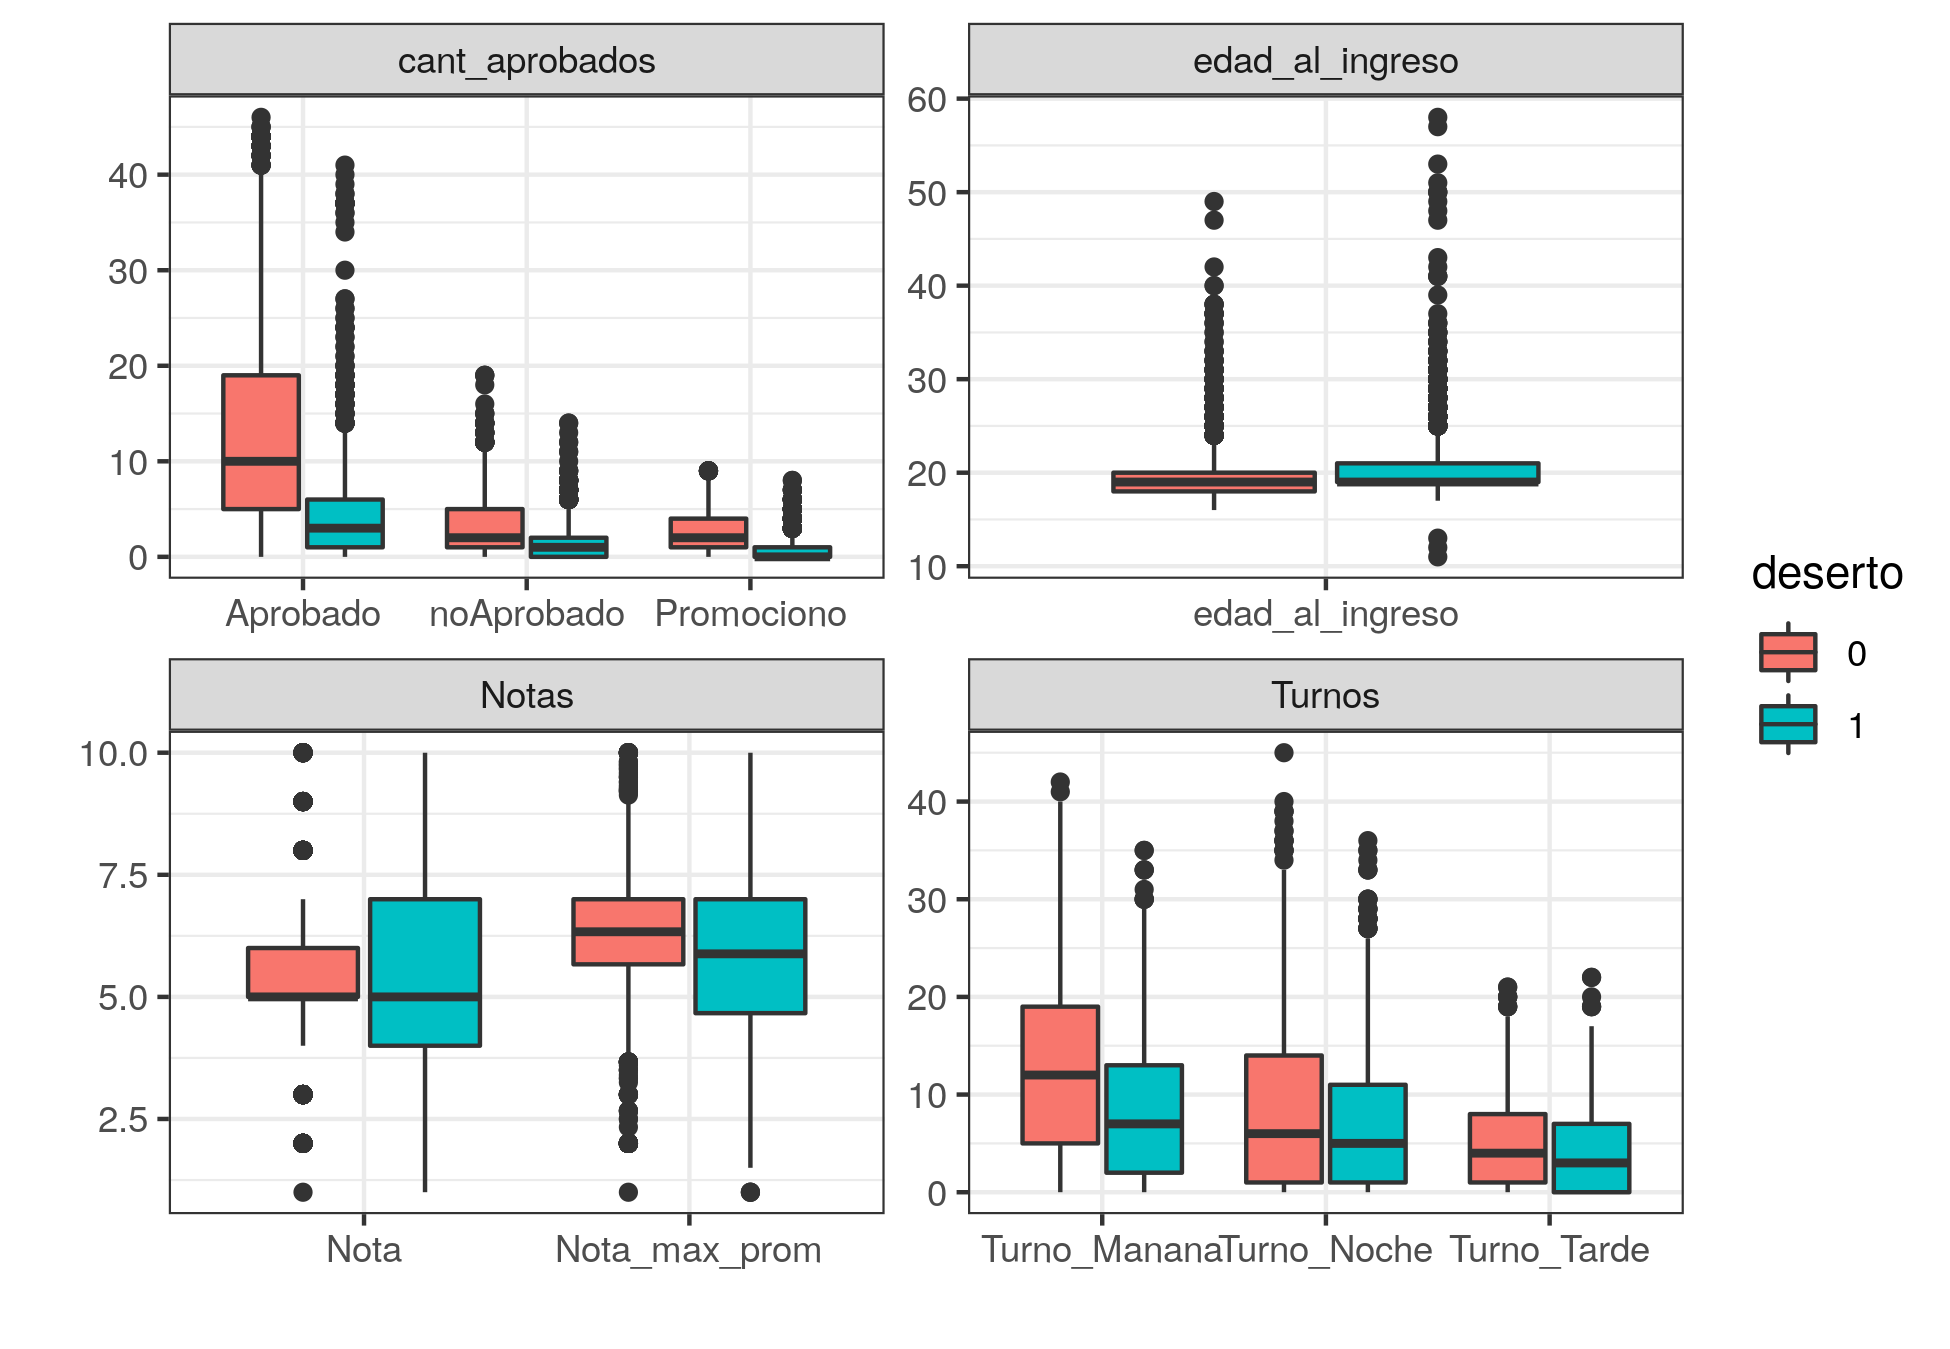
\includegraphics{imagenes/imagenes/gg_explo_tablon_grupo.png}
	%\includegraphics[width=0.25\textwidth]{mesh}
	\caption{Análisis Univariado por grupos}
	\label{fig:tablon_boxplot_grupo}
\end{figure}

\begin{figure}[!htb]
	\centering
	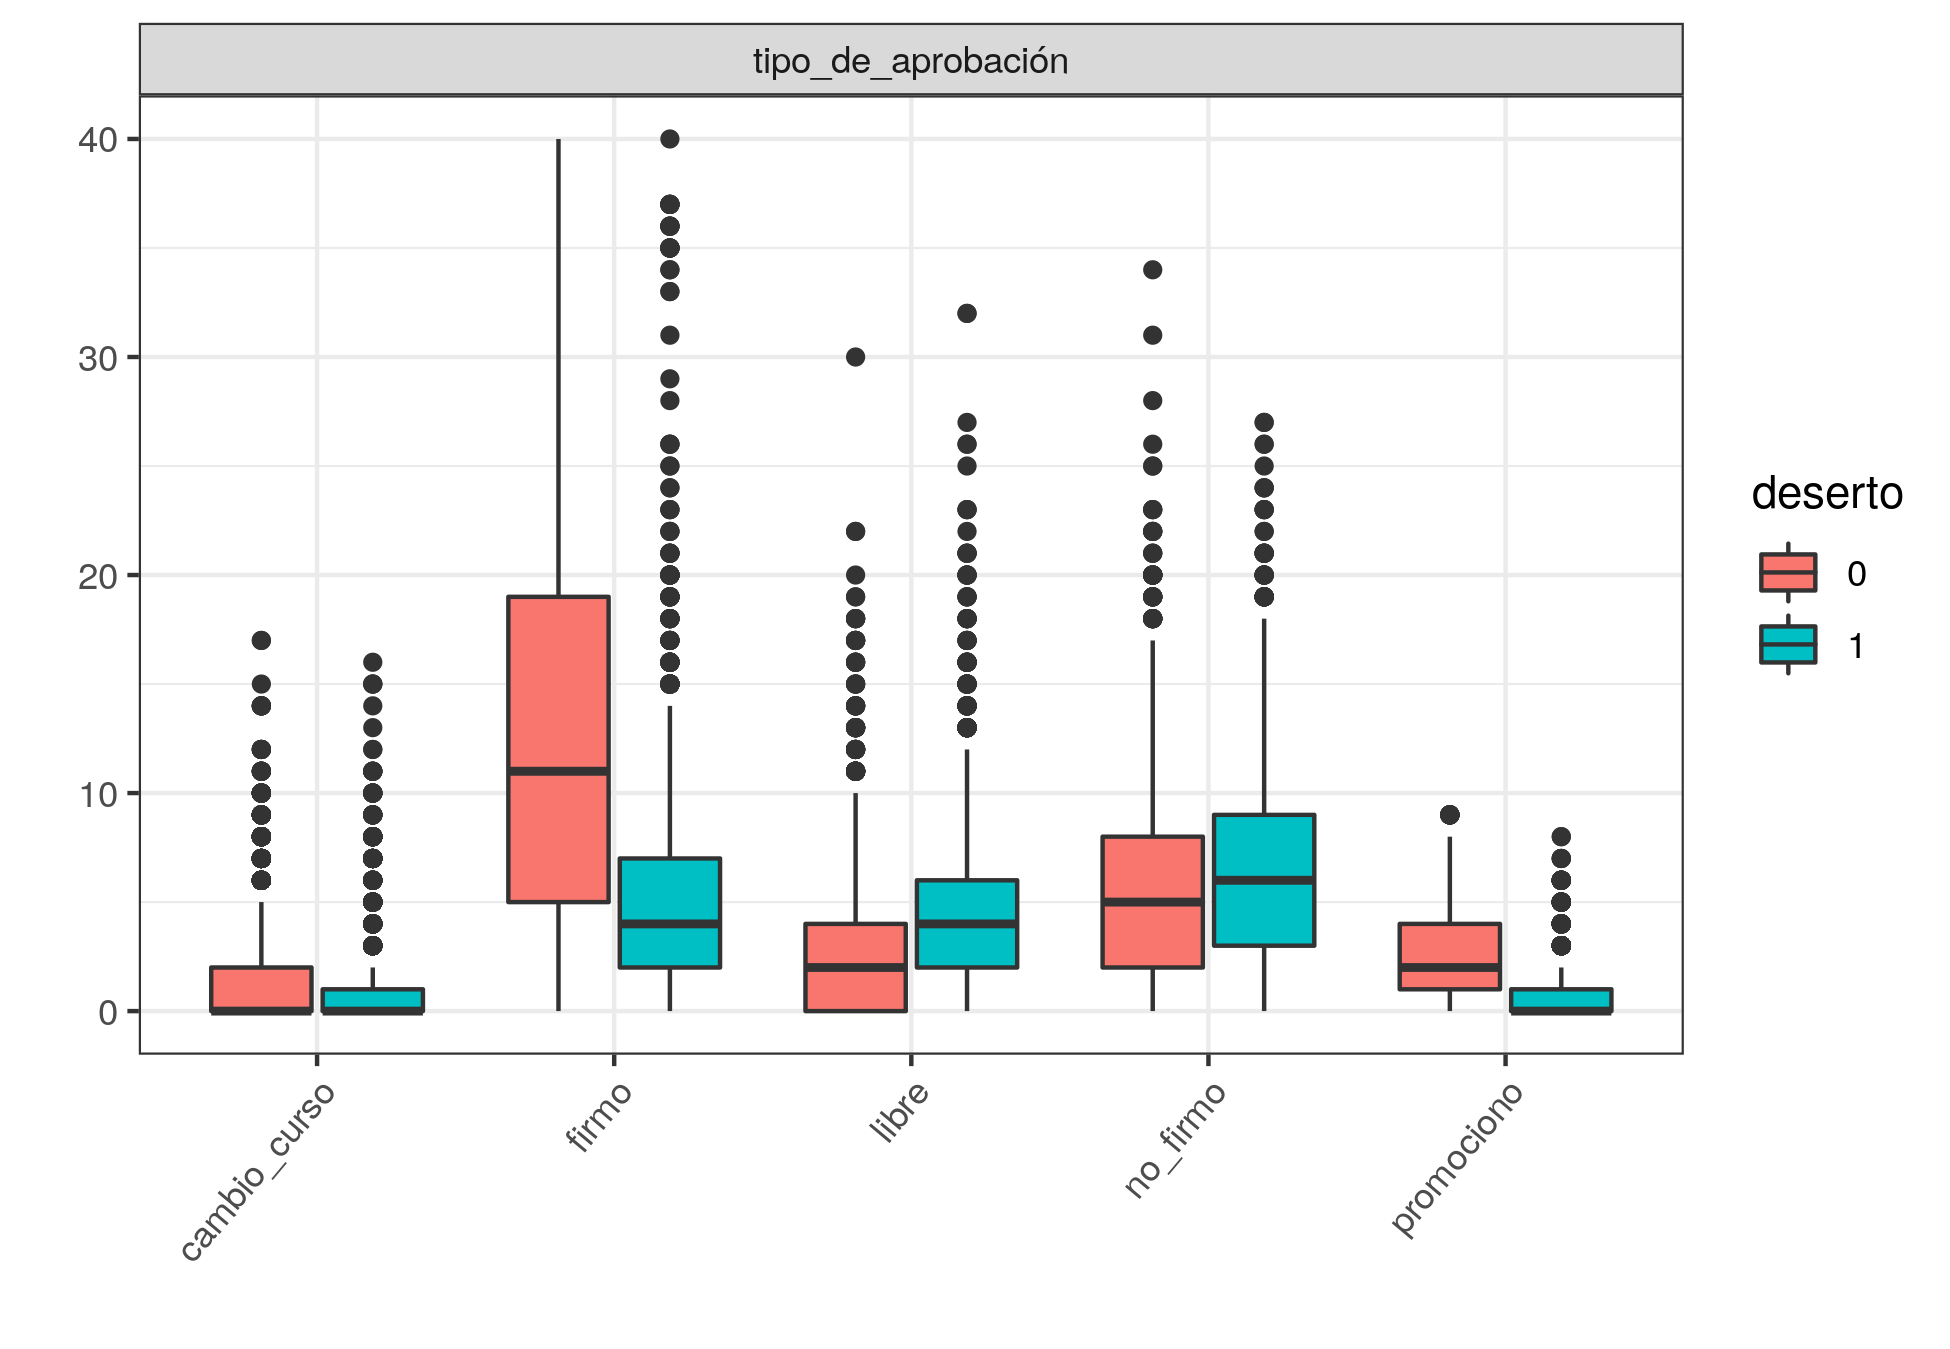
\includegraphics{imagenes/imagenes/gg_explo_tablon_tipo_aprob.png}
	%\includegraphics[width=0.25\textwidth]{mesh}
	\caption{Análisis Univariado por Tipo de Aprobación}
	\label{fig:tablon_boxplot_tipoAprobacion}
\end{figure}

\begin{figure}[!htb]
	\centering
	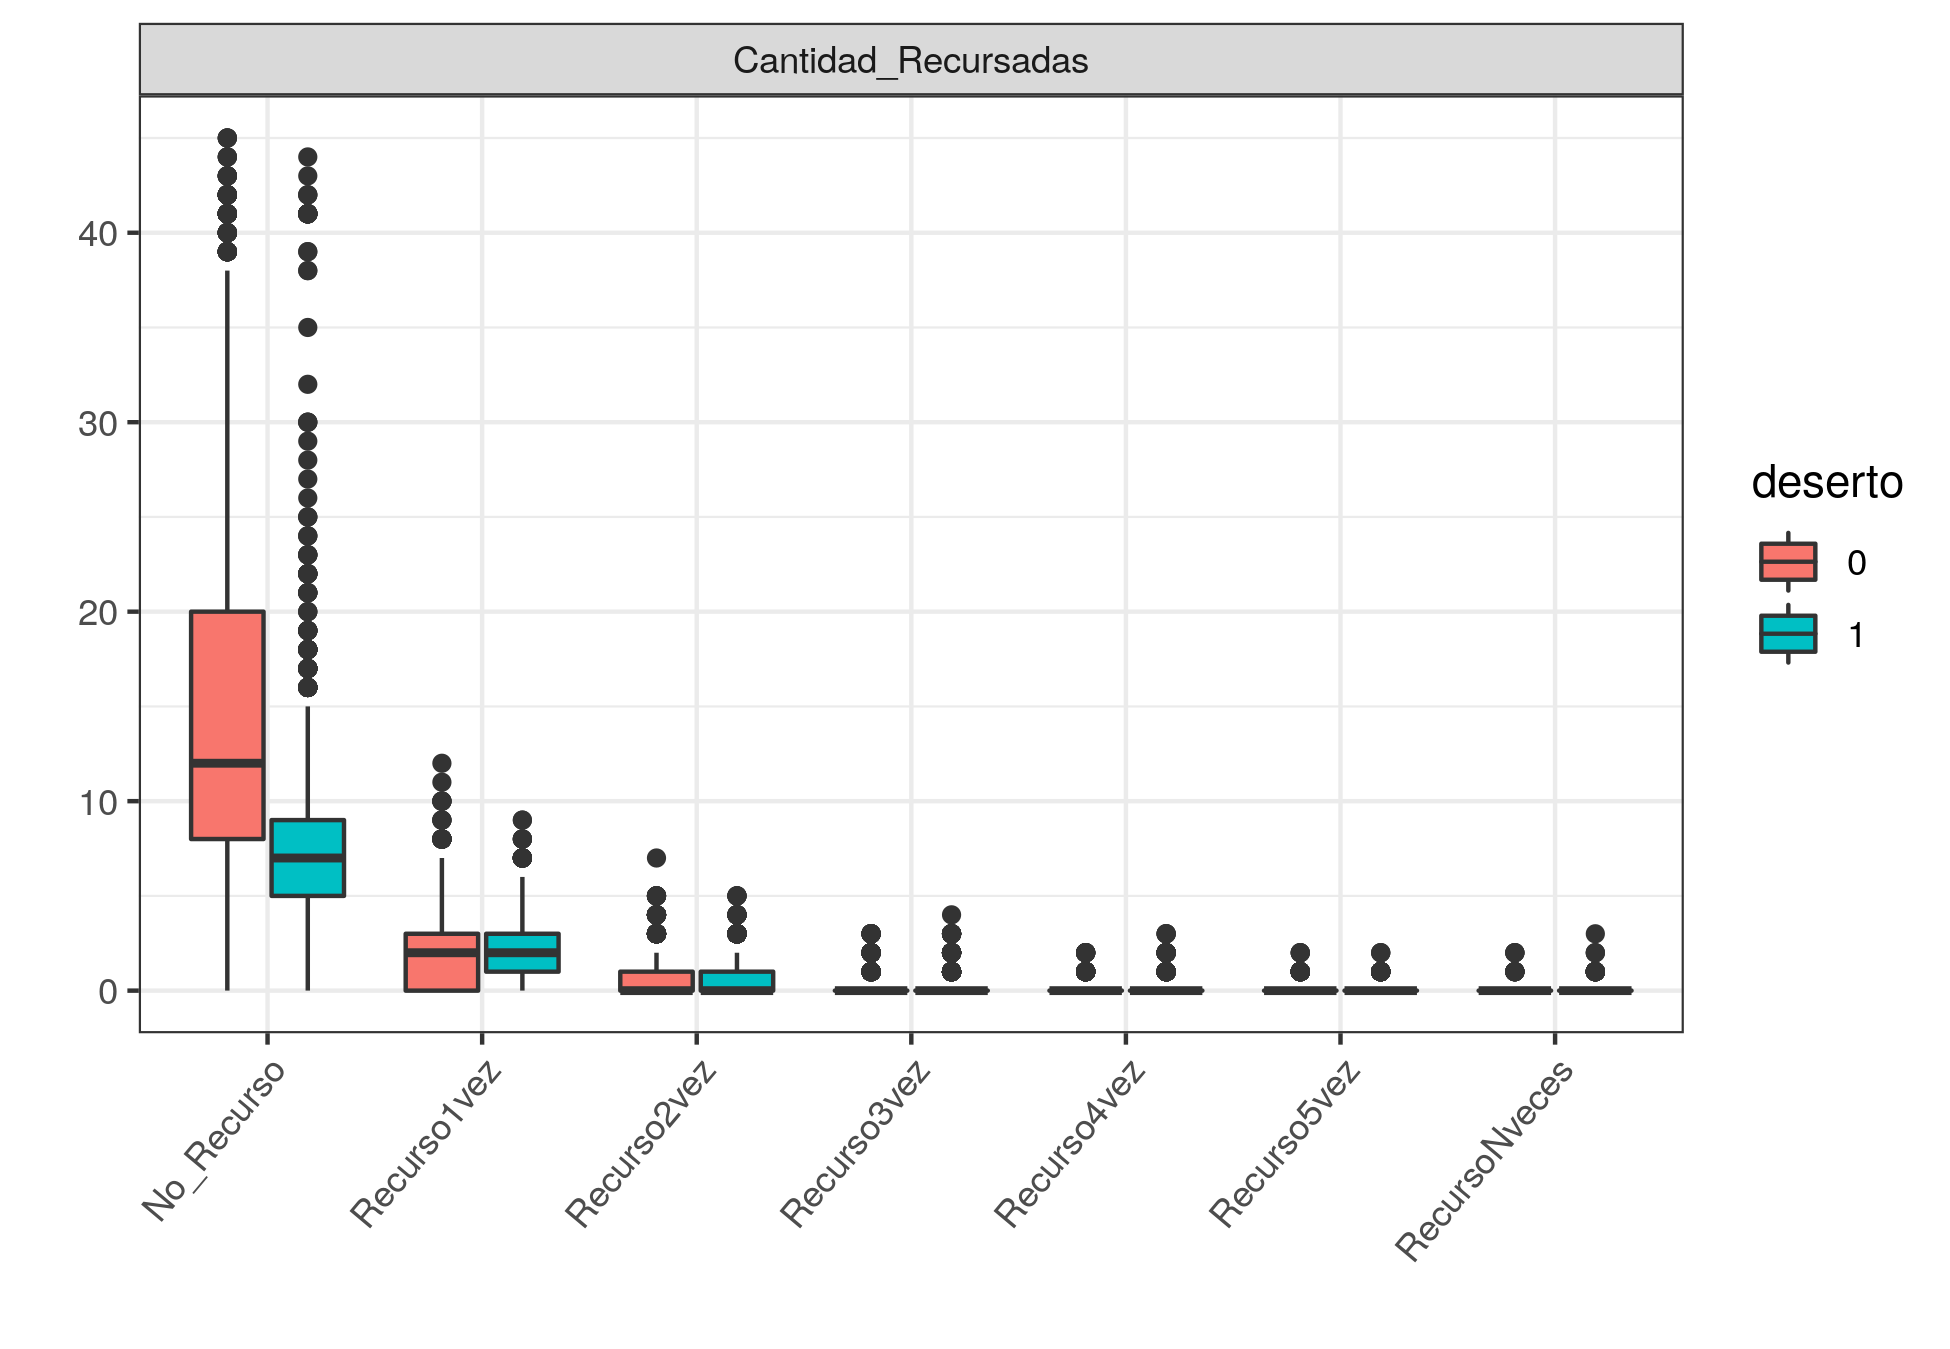
\includegraphics{imagenes/imagenes/gg_explo_tablon_tipo_recur.png}
	%\includegraphics[width=0.25\textwidth]{mesh}
	\caption{Análisis Univariado por tipo de resursada}
	\label{fig:tablon_boxplot_tipoRecursada}
\end{figure}

\clearpage

\hypertarget{observaciones}{%
	\paragraph{Observaciones}\label{observaciones}}

De las tablas y gráficos anteriores podemos extraer la siguiente
información:

\begin{itemize}
	\item
	El dataset se encuentra balanceado. 43.88 \% de los alumnos del
	dataset desertó mientras que el 56.12 \% sigue en carrera.
	\item
	La variable \textbf{EsTecnico} tiene un 13.32\% de datos nulos.
	Dependiendo el método que se use podrá tolerarse o no. En los casos
	que no se pueda tolerar, se tendrá que imputar algún valor o se podrá
	optar por descartar la variable.
	\item
	El valor mínimo de la variable \textbf{edad\_al\_ingreso} es 11. Un
	valor muy bajo y puede tratarse de un error. Se analizaron la cantidad
	de casos que existen en que esta variable tiene un valor menor a 17,
	que es la mínima edad que podría entrar un estudiante a la universidad
	respetando todos los ciclos lectivos sin adelantar ninguno de las
	etapas de estudio anteriores, y dicho valor es de 4 observaciones. Las
	cuales representan una cantidad insignificante respecto del total de
	observaciones 4558 (0.06\%). Por lo tanto al no poder verificarlo por
	el momento se decide dejarlo.
\end{itemize}

\hypertarget{correlaciuxf3n-entre-todas-las-variables}{%
	\paragraph{Correlación entre todas las
		variables}\label{correlaciuxf3n-entre-todas-las-variables}}

%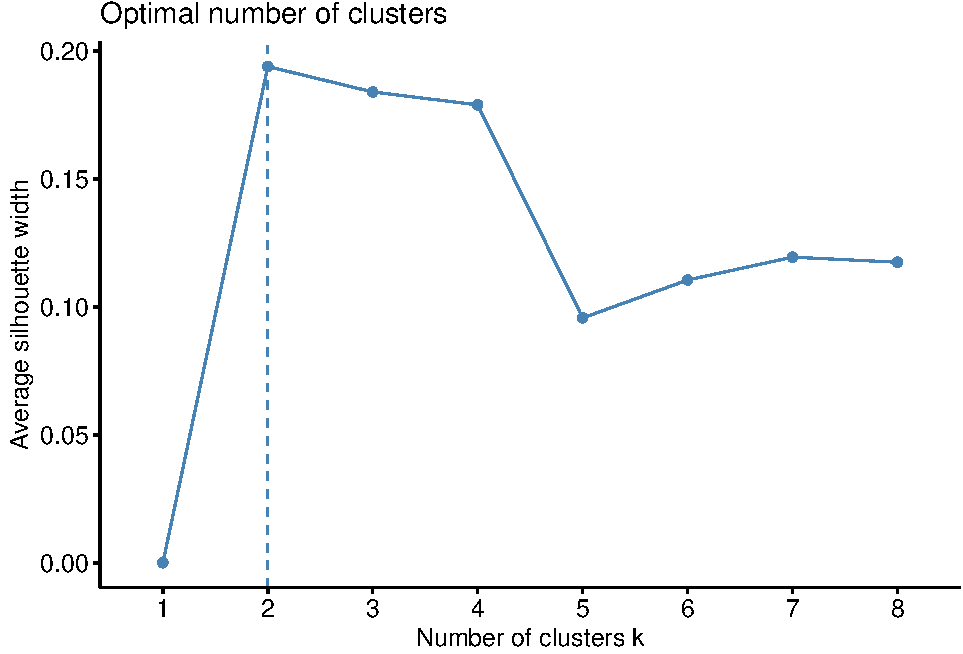
\includegraphics{Analisis_tablon_baseline_2009_files/figure-latex/unnamed-chunk-15-1.pdf}

\begin{figure}[!htb]
	\centering
	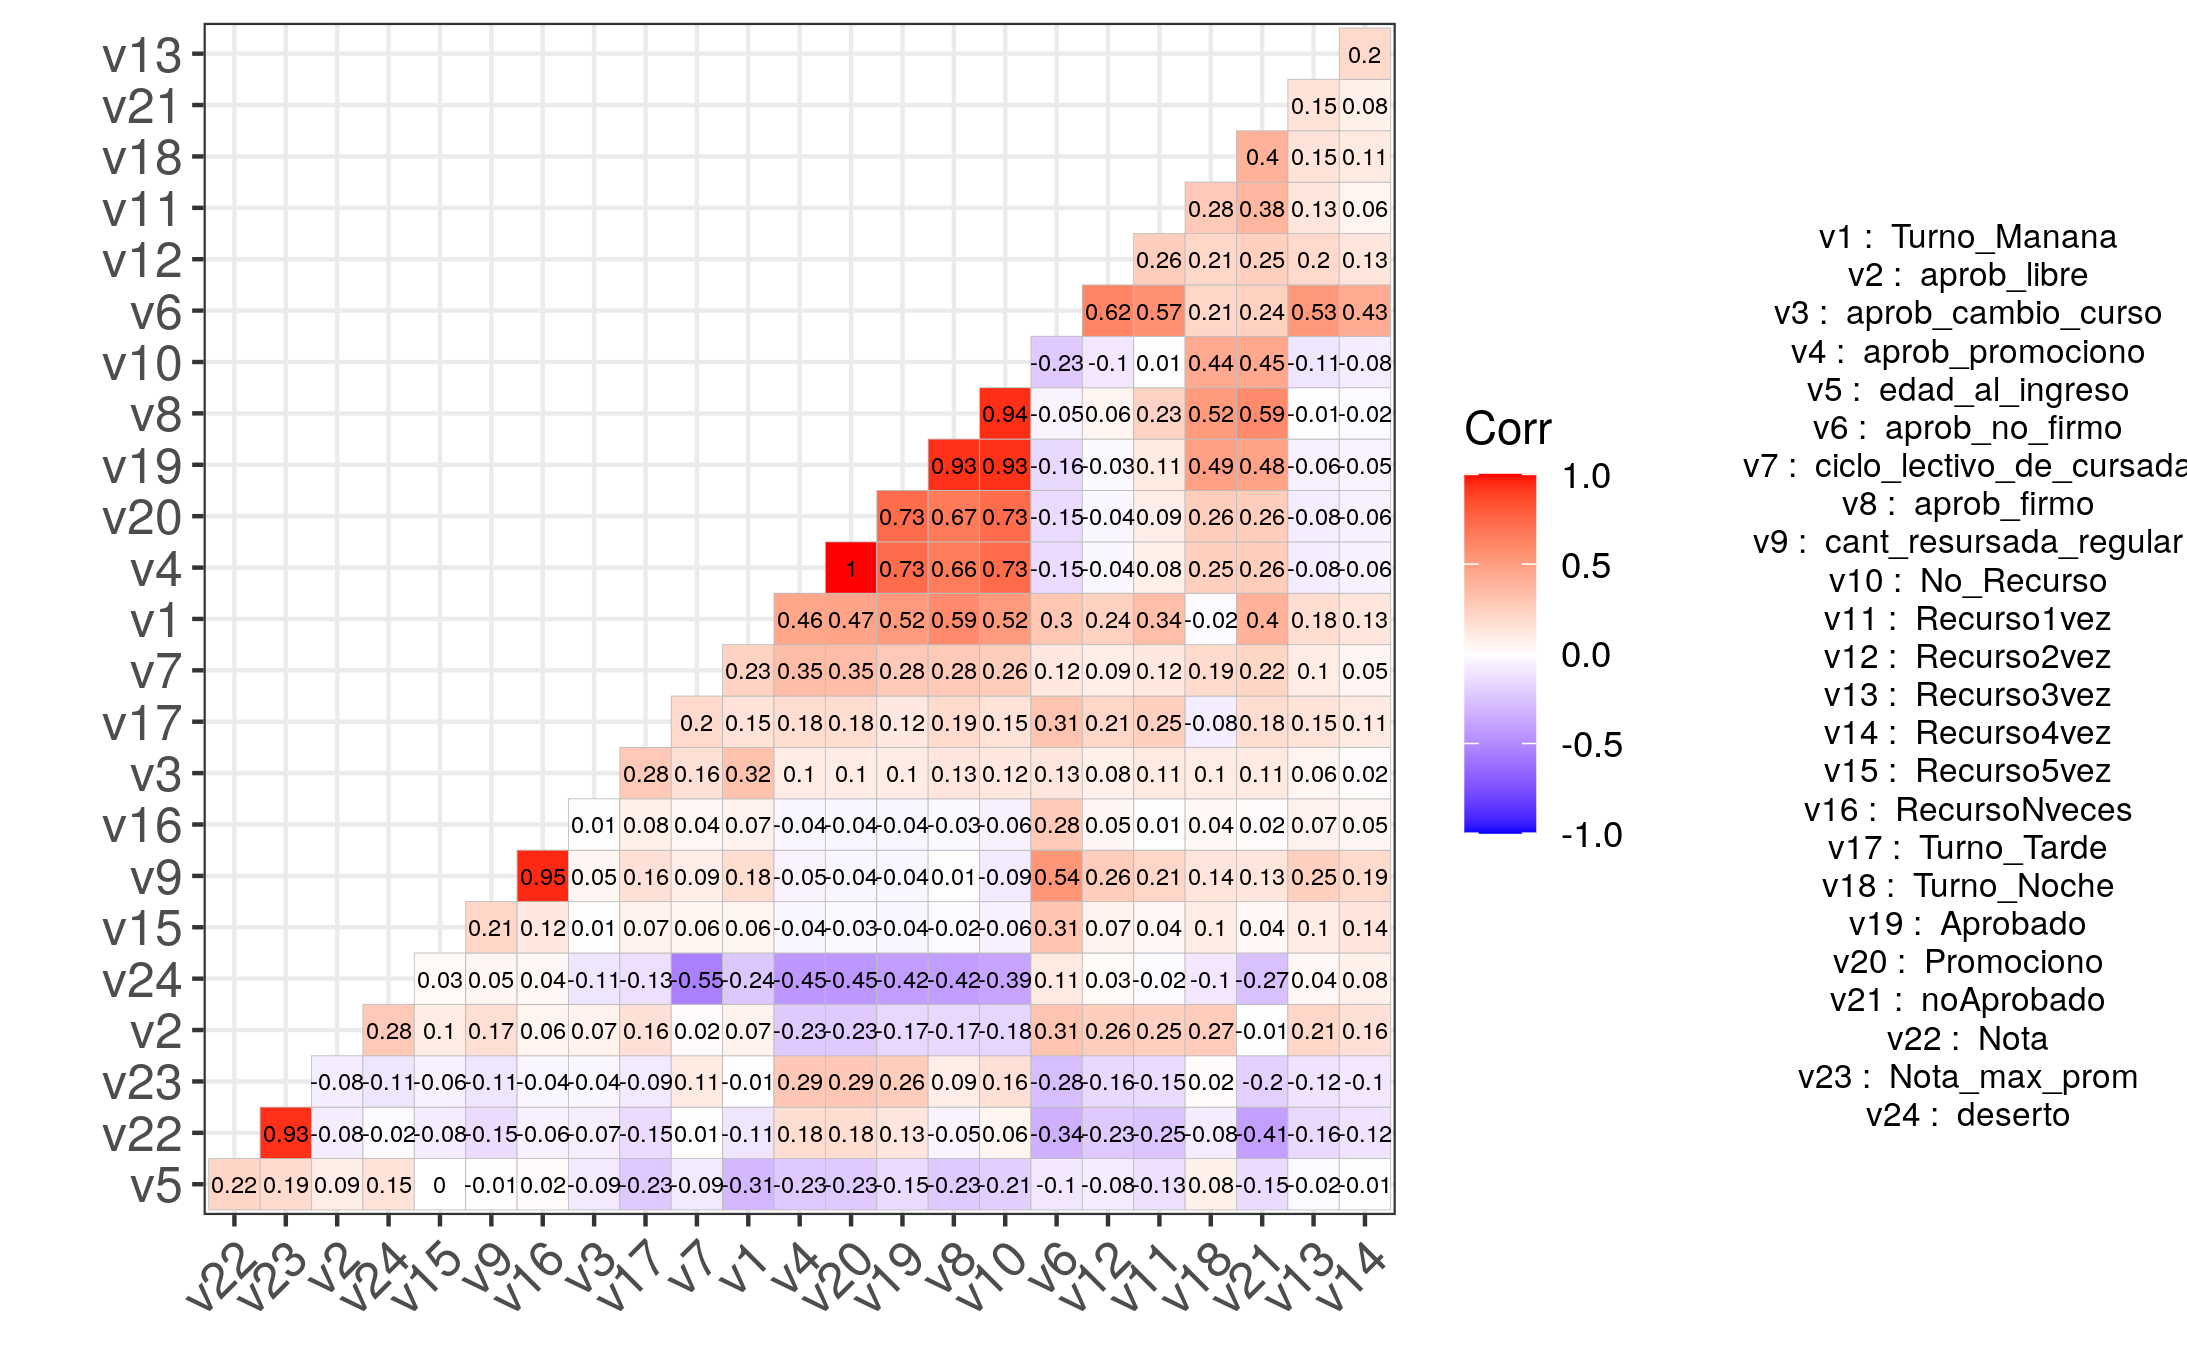
\includegraphics[width=0.98\textwidth]{imagenes/imagenes/gg_corr_todas_variables_leyenda.png}
	%\includegraphics[width=0.25\textwidth]{mesh}
	\caption{Análisis Univariado por tipo de resursada}
	\label{fig:tablon_correlacion}
\end{figure}

\hypertarget{correlaciuxf3n-entre-las-variables-y-la-clase}{%
	\paragraph{Correlación entre las variables y la
		clase}\label{correlaciuxf3n-entre-las-variables-y-la-clase}}

Si bien la clase es categórica y la mayoría de las variables son
numéricas, podemos convertir la clase en númerica convirtiendo los casos
positivos en 1 y los negativos en 0. De esta forma podemos analizar por
el coeficiente de correlación si es que existen variables predictoras
que sigan o se acerquen al comportamiento de la clase. Como veremos en
la sigueinte tabla, no hay una relación muy directa entre cada variable
individual con la clase convertid en numérica.

\begin{table}[!h]
	
	\caption{\label{tab:tablon_correl_clase}Correlacion con la clase}
	\centering
	\begin{tabular}[t]{llr}
		\toprule
		\rowcolor{black}  \multicolumn{1}{c}{\textcolor{white}{\textbf{nombrefila}}} & \multicolumn{1}{c}{\textcolor{white}{\textbf{nombrecolumna}}} & \multicolumn{1}{c}{\textcolor{white}{\textbf{correl}}}\\
		\midrule
		\rowcolor{gray!6}  deserto & ciclo\_lectivo\_de\_cursada & -0.55\\
		deserto & tipo\_de\_aprobacion\_promociono & -0.45\\
		\rowcolor{gray!6}  deserto & Promociono & -0.45\\
		deserto & tipo\_de\_aprobacion\_firmo & -0.42\\
		\rowcolor{gray!6}  deserto & Aprobado & -0.42\\
		\addlinespace
		deserto & cant\_recursada\_regular\_No\_Recurso & -0.39\\
		\rowcolor{gray!6}  deserto & tipo\_de\_aprobacion\_libre & 0.28\\
		deserto & noAprobado & -0.27\\
		\rowcolor{gray!6}  deserto & Turno\_Manana & -0.24\\
		deserto & edad\_al\_ingreso & 0.15\\
		\addlinespace
		\rowcolor{gray!6}  deserto & Turno\_Tarde & -0.13\\
		deserto & tipo\_de\_aprobacion\_no\_firmo & 0.11\\
		\rowcolor{gray!6}  deserto & tipo\_de\_aprobacion\_cambio\_curso & -0.11\\
		deserto & Nota\_max\_prom & -0.11\\
		\rowcolor{gray!6}  deserto & Turno\_Noche & -0.10\\
		\addlinespace
		deserto & cant\_recursada\_regular\_Recurso4vez & 0.08\\
		\rowcolor{gray!6}  deserto & cant\_resursada\_regular & 0.05\\
		deserto & cant\_recursada\_regular\_Recurso3vez & 0.04\\
		\rowcolor{gray!6}  deserto & cant\_recursada\_regular\_RecursoNveces & 0.04\\
		deserto & cant\_recursada\_regular\_Recurso5vez & 0.03\\
		\addlinespace
		\rowcolor{gray!6}  deserto & cant\_recursada\_regular\_Recurso2vez & 0.03\\
		deserto & Nota & -0.02\\
		\rowcolor{gray!6}  deserto & cant\_recursada\_regular\_Recurso1vez & -0.02\\
		\bottomrule
	\end{tabular}
\end{table}



\subsubsection{Análisis de Variables Importantes}\label{analisis-var_importantes}

Incluir un exceso de variables en el modelo suele traer aparejado una disminución de la capacidad predictiva de un modelo cuando se expone a nuevos datos (overfitting). \\
Se realizan múltiples evaluaciones de modelos de RandomForest con bootstrapping generados mediante incorporación y eliminación de predictores con la finalidad de identificar la combinación óptima. Este análisis de realiza unicamente con el datset de train para que los valores de test no influyan en este procedimiento.\\

En la tabla \ref{tab:top_10_rfe_accuracy} se detallan los mejores 10 modelos obtenidos a partir de toda la combinación posibles. Puede observarse que el mejor modelo a juzgar por la métrica Accuracy es el que se entreno solamente con 10 predictores de los 25 que cuenta el datset completo. Dichos predictores son: 
``ciclo\_lectivo\_de\_cursada",``tipo\_de\_aprobacion\_libre", ``Turno\_Noche", ``tipo\_de\_aprobacion\_no\_firmo", ``Aprobado", ``Turno\_Tarde", ``Nota\_max\_prom", ``tipo\_de\_aprobacion\_firmo", ``Turno\_Manana" y ``cant\_resursada\_regular".\\

Asimismo, en la figura \ref{fig:rfe_evolucion_accuracy} se puede observar la evolución de la mátrica accuracy en función de la cantidad de variables que toma el modelo. La dispersión en este caso está asociado a los distintos valores de accuracy que tiene cada modelo ejecutado en cross validation como así también está conplemtado todas las combinaciones de variables posibles con la cantidad que marca el eje x.\\
Ademas de que al usar menos variables se necesita menos poder de computo, es más fácil la interpretación que se podrá hacer y tendremos una menor dispersión final.

\begin{table}[!h]
	
	\caption{\label{tab:top_10_rfe_accuracy}Top 10 Modelos con cantidad de variables seleccionadas según Accuracy}
	\centering
	\begin{tabular}[t]{rrr}
		\toprule
		\rowcolor{black}  \multicolumn{1}{c}{\textcolor{white}{\textbf{Variables}}} & \multicolumn{1}{c}{\textcolor{white}{\textbf{media\_accuracy}}} & \multicolumn{1}{c}{\textcolor{white}{\textbf{media\_kappa}}}\\
		\midrule
		\rowcolor{gray!6}  10 & 0.8388631 & 0.6690887\\
		18 & 0.8385668 & 0.6687514\\
		\rowcolor{gray!6}  11 & 0.8381883 & 0.6678640\\
		19 & 0.8381476 & 0.6679149\\
		\rowcolor{gray!6}  17 & 0.8380654 & 0.6677621\\
		\addlinespace
		9 & 0.8377655 & 0.6670357\\
		\rowcolor{gray!6}  23 & 0.8368520 & 0.6655250\\
		20 & 0.8360972 & 0.6636373\\
		\rowcolor{gray!6}  15 & 0.8360919 & 0.6637290\\
		22 & 0.8355010 & 0.6625480\\
		\bottomrule
	\end{tabular}
\end{table}

\begin{figure}[!htb]
	\centering
	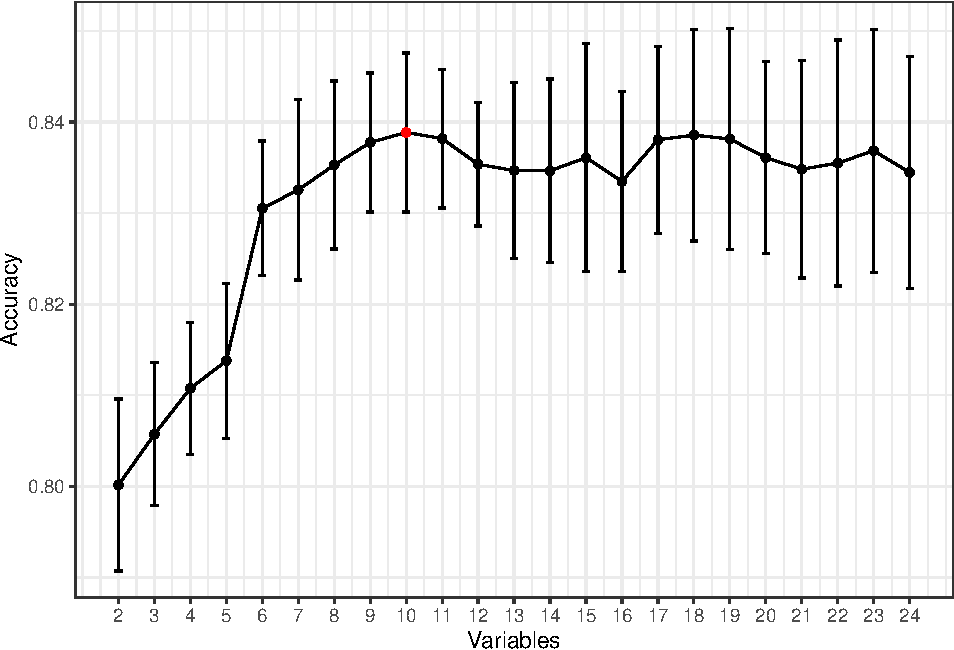
\includegraphics{imagenes/variables/rfe_evolucion_accuracy-1.pdf}
	%\includegraphics[width=0.25\textwidth]{mesh}
	\caption{Evolución de l Métrica Accuracy en función de la cantidad de variables usadas por el modelo}
	\label{fig:rfe_evolucion_accuracy}
\end{figure}

\paragraph{influencia de variables}
Tras ajustar cada uno de estos modelos, se recalcula la influencia de cada variable. De esta forma, para cada tamaño de modelo, se obtiene un ranking de la importancia promedio de las variables. Los resultados se pueden observar en \ref{tab:tf_rfe_influencia_variables} y \ref{fig:rfe_influencia_var} donde existe una variable que claramente influye mucho mas en los resultados en comparación con los otros predictores.

\begin{table}[!h]
	
	\caption{\label{tab:tf_rfe_influencia_variables}Influencia de variables en el resultado}
	\centering
	\begin{tabular}[t]{lrr}
		\toprule
		\rowcolor{black}  \multicolumn{1}{c}{\textcolor{white}{\textbf{var}}} & \multicolumn{1}{c}{\textcolor{white}{\textbf{media\_influencia}}} & \multicolumn{1}{c}{\textcolor{white}{\textbf{sd\_influencia}}}\\
		\midrule
		\rowcolor{gray!6}  ciclo\_lectivo\_de\_cursada & 89.84029 & 2.9668673\\
		tipo\_de\_aprobacion\_libre & 46.34285 & 2.2575528\\
		\rowcolor{gray!6}  Turno\_Noche & 38.07504 & 1.7175035\\
		tipo\_de\_aprobacion\_no\_firmo & 38.05189 & 1.5399760\\
		\rowcolor{gray!6}  Aprobado & 35.80734 & 1.1307306\\
		\addlinespace
		Turno\_Tarde & 35.67467 & 1.5035133\\
		\rowcolor{gray!6}  tipo\_de\_aprobacion\_firmo & 35.28770 & 0.6960169\\
		Nota\_max\_prom & 35.14407 & 2.3991503\\
		\rowcolor{gray!6}  Turno\_Manana & 34.30645 & 1.5999039\\
		cant\_resursada\_regular & 32.25476 & 1.1929776\\
		\addlinespace
		\rowcolor{gray!6}  edad\_al\_ingreso & 31.90459 & 0.1024266\\
		\bottomrule
	\end{tabular}
\end{table}

\begin{figure}[!htb]
	\centering
	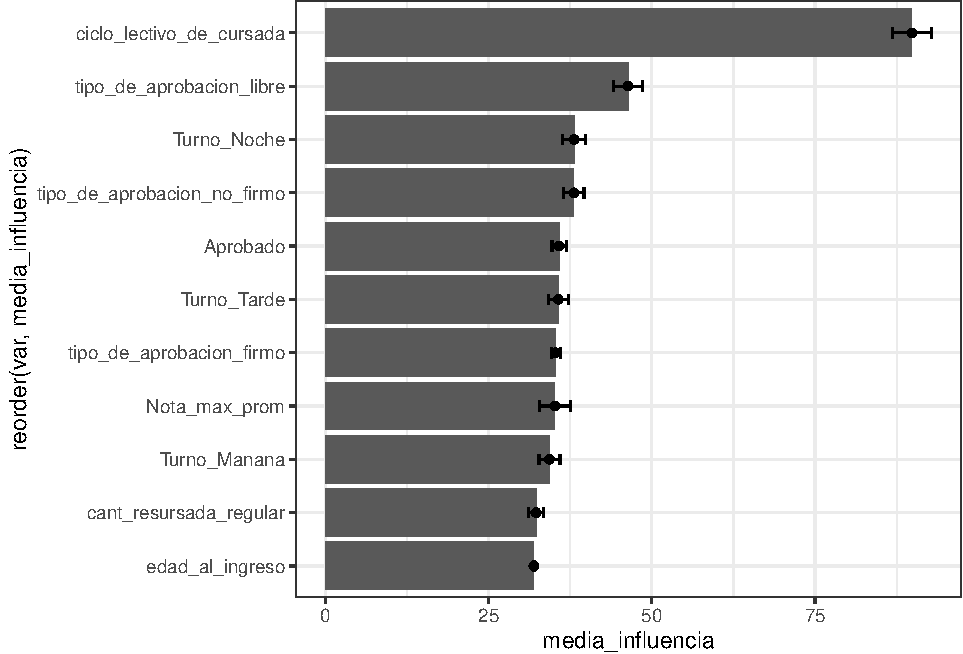
\includegraphics{imagenes/variables/influencia_de_variables-1.pdf}
	%\includegraphics[width=0.25\textwidth]{mesh}
	\caption{Influencia de las variables mas importances sobre el resultado}
	\label{fig:rfe_influencia_var}
\end{figure}

\clearpage

